% document formatting
\documentclass[10pt]{article}
\usepackage[utf8]{inputenc}
\usepackage[left=1in,right=1in,top=1in,bottom=1in]{geometry}
\usepackage[T1]{fontenc}
\usepackage{xcolor}

% math symbols, etc.
\usepackage{amsmath, amsfonts, amssymb, amsthm}

% lists
\usepackage{enumerate}

% images
\usepackage{graphicx} % for images
\usepackage{multirow}

% code blocks
\usepackage{minted, listings} 

% verbatim greek
\usepackage{alphabeta}

\graphicspath{{./assets/images}}

\newcommand{\solution}{\textbf{Solution:}} 
\newcommand{\example}{\textbf{Example: }}
\newcommand{\sinc}{\text{sinc}}
\newcommand{\rect}{\text{rect}}

\title{EC ENGR 102 Week 6}

\author{Aidan Jan}
\date{\today}

\begin{document}
\maketitle

\subsection*{Proof of the Convolution Theorem}
\begin{align*}
    \mathcal{F}[(f_1 * f_2)(t)] &= \int_{-\infty}^\infty \left(\int-{-\infty}^\infty f_1(\tau) f_2(t - \tau) \text{d}\tau\right) e^{-j\omega t} \text{d}t\\
    &= \int_{-\infty}^\infty f_1(t) \int_{-\infty}^\infty f_2(t-\tau) e^{-j\omega t} \text{d}t \:\text{d}\tau\\
    &= \int_{-\infty}^\infty f-1(t) \left[e^{-j\omega \tau} F_2(j\omega)\right] \text{d}\tau\\
    &= F_2(j\omega) \cdot \int_{-\infty}^\infty f_1(\tau) e^{-j\omega \tau} \text{d}\tau\\
    &= F_2(j\omega) \cdot F_1(j\omega)
\end{align*}

\subsubsection*{Example}
What is the Fourier transform of the unit triangle,
\[\triangle(t)=\begin{cases} 1-|t|& |t|<1 \\ 0 & \text{otherwise}\end{cases}\]

\subsection*{Duality of the Fourier Transform}
If $\mathcal{F}[f(t)] = F(j\omega)$, then
\[\boxed{F(t) \Longleftrightarrow 2\pi f(-j\omega)}\]
This expression may be opaque at first.  What this is saying is that if I take a Fourier transform pair, I can find the dual pair by replacing all the $\omega$'s with $t$'s in $F(j\omega)$ and all the $t$'s with $-\omega$'s in $f(t)$.  After scaling by $2\pi$, this results in another Fourier transform pair.\\\\
Essentially, every Fourier transform pair we derive really gives us two Fourier transform pairs.

\subsubsection*{Duality Proof}
To show this, recognize that as
\[f(t) = \frac{1}{2\pi} \int_{-\infty}^\infty F(j\omega) e^{j\omega t} \text{d}\omega\]
then
\[2\pi f(-t) = \int_{-\infty}^\infty F(j\omega) e^{-j\omega t} \text{d}\omega\]
Now, the right hand side of this equation is the Fourier transform of $F(j\omega)$ with the roles of $\omega$ and $t$ reversed.  Hence, $2\pi f(-t)$ is the Fourier transform of $F(j\omega)$ and after we swap the $\omega$ and the $t$'s, we arrive at the duality result.

\subsubsection*{Duality Examples}
\begin{itemize}
    \item Since $\rect(t) \Longleftrightarrow \sinc(\omega/2\pi)$, then
    \begin{align*}
        \sinc(t/2\pi) &\Longleftrightarrow 2\pi \rect(-\omega)\\
        &\hspace{0.18cm}= 2\pi \rect(\omega)
    \end{align*}
    Thus, we have that $\sinc(t/2\pi) \Longleftrightarrow 2\pi \rect(\omega)$.
    \item Since
    \[e^{-at} u(t) \Longleftrightarrow \frac{1}{a+j\omega}\]
    then 
    \[\frac{1}{a+jt} \Longleftrightarrow 2\pi e^{a\omega} u(-\omega)\]
\end{itemize}

\subsection*{Frequency Domain Convolution}
The frequency domain convolution theorem is that for $f_1(t) \Longleftrightarrow F_1(j\omega)$ and $f_2(t) \Longleftrightarrow F_2(j\omega)$, then
\[\boxed{\mathcal{F}[f_1(t)f_2(t)] = \frac{1}{2\pi} \int_{-\infty}^\infty F_1(jv) F_2(j(\omega - v)) \text{d}v}\]
We typically write this as:
\[\boxed{\mathcal{F}[f_1(t)f_2(t)] = \frac{1}{2\pi} (F_1 * F_2)(j\omega)}\]
but note that the convolution is with respect to $\omega$, not $j\omega$.  (Remember that $j$ is constant!)\\\\
This means that multiplication in the time domain is convolution in the frequency domain.  This proof is very similar to the time domain proof.

\subsection*{Modulation: duality of time-shifting}
Dual intuition: Time shift in the time domain is multiplication by a complex exponential in frequency domain.  Thus, multiplication by a complex exponential in the time domain ought be a shift in the frequency domain.\\\\
Recall that:
\[\boxed{\mathcal{F}[f(t-\tau)] = e^{-j\omega \tau} F(j\omega)}\]
Another FT pair (derived later) is
\[\mathcal{F}[f(t)e^{j\omega_0 t} = F(j(\omega - \omega_0))]\]
Using linearity, we also see that:
\begin{align*}
    \mathcal{F}[f(t)\cos(\omega_0 t)] &= \frac{1}{2}(F(j(\omega - \omega_0)) + F(j(\omega + \omega_0)))\\
    \mathcal{F}[f(t)\sin(\omega_0 t)] &= \frac{1}{2j}(F(j(\omega - \omega_0)) - F(j(\omega + \omega_0)))
\end{align*}
To prove the modulation result, note that if $\mathcal{F}[f(t)] = F(j\omega)$ then
\begin{align*}
    \mathcal{F}[f(t)e^{j\omega_0 t}] &= \int_{-\infty}^\infty f(t)e^{j\omega_0 t} e^{-j\omega t} \text{d}t\\
    &= \int_{-\infty}^\infty f(t) e^{-j(\omega-\omega_0)t} \text{d}t\\
    &= F(j(\omega-\omega_0))
\end{align*}
To get the cosine and sine results, we note that e.g., for cosine,
\[\cos(\omega_0 t) = \frac{1}{2}\left(e^{j\omega_0 t} + e^{-j\omega_0 t}\right)\]
From here, we can use linearity to compute the Fourier transform.
\end{document}

\subsubsection*{Fourier Transform of a Modulated Signal}
A major component of communications has to do with \textit{modulation}. For example, AM and FM radio are amplitude modulation and frequency modulation respectively.  AM radio involves multiplying $f(t)$, the signal you wish to transmit, with a complex exponential at a carrier frequency, $\omega_0$.  This frequency, $\omega_0$, is the frequency you dial in your car to get AM radio.\\\\
Here are three ways to modulate a signal: If $\mathcal{F}[f(t)] = F(j\omega)$, then
\begin{align*}
    \mathcal{F}[f(t) e^{j\omega_0 t}] &= F(j(\omega - \omega_0))\\
    \mathcal{F}[f(t) \cos(\omega_0 t)] &= \frac{1}{2} (F(j(\omega - \omega_0)) + F(j(\omega + \omega_0)))\\
    \mathcal{F}[f(t) \sin(\omega_0 t)] &= \frac{1}{2j} (F(j(\omega - \omega_0)) - F(j(\omega + \omega_0)))
\end{align*}
Typically, modulation is done through multiplication by $\cos(\omega_0 t)$.  Modulation is dual to the time shift Fourier transform.\\\\
What modulation intuitively does is take $F(j\omega)$ and create replicas at $\pm \omega_0$.\\\\
Below, we show what modulation does.  We take a signal (here a rect) and multiply it by a cosine with $\omega_0 = 30\pi$.  This is denoted in red in the plot below.
\begin{center}
    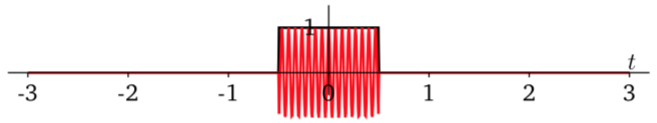
\includegraphics[scale=0.8]{W6_1.png}
\end{center}
The spectrum takes the FT of our signal (i.e., a sinc) and creates replicas at $\pm 30\pi$.
\begin{center}
    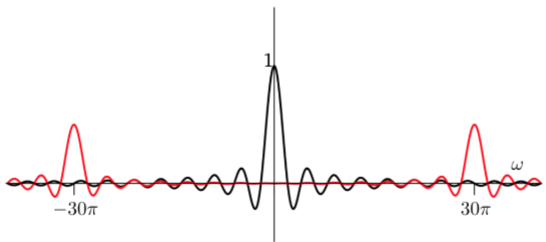
\includegraphics[scale=0.8]{W6_2.png}
\end{center}
From here, you can gain some intuition for why different radio stations use different frequencies.  They're given these frequencies to transmit whatever signals they like; each radio station occupies a different part of the spectrum!

\subsection*{Parseval's Theorem}
Recall that the energy for a signal, $f(t)$, is given by
\[\Epsilon_f = \int_{-\infty}^\infty |f(t)|^2 \text{d}t\]
Parseval's theorem states that the energy of the signal and its Fourier transform are equal up to a scaling factor of $2\pi$, i.e., 
\[\boxed{\int_{-\infty}^\infty |f(t)|^2 \text{d}t = \frac{1}{2\pi} \int_{-\infty}^\infty |F(j\omega)|^2 \text{d}\omega}\]
To see this,
\begin{align*}
    \Epsilon_f &= \int_{-\infty}^\infty |f(t)|^2 \text{d}t\\
    &= \int_{-\infty}^\infty f(t) f^*(t) \text{d}t\\
    &= \int_{-\infty}^\infty f(t) \left(\frac{1}{2\pi} \int_{-\infty}^\infty F(j\omega) e^{j\omega t} \text{d}\omega\right)^* \text{d}t\\
    &= \frac{1}{2\pi} \int_{-\infty}^\infty F^*(j\omega)\left(\int_{-\infty}^\infty f(t) e^{-j\omega t} \text{d}t\right) \text{d}\omega\\
    &= \frac{1}{2\pi} \int_{-\infty}^\infty F^*(j\omega) F(j\omega) \text{d}\omega\\
    &= \frac{1}{2\pi} \int_{-\infty}^\infty |F(j\omega)|^2 \text{d}\omega
\end{align*}
Like in Fourier series, Parseval's theorem can be used to make integrals a lot easier.  Say you were asked to calculate:
\[\int_{-\infty}^\infty \sinc^2(t) \text{d}t\]
Since $\sinc(t) \Longleftrightarrow \rect(\omega/2\pi)$, then
\[\int_{-\infty}^\infty \sinc^2(t) \text{d}t\]
[FILL]

\subsubsection*{Fourier Transform of the Derivative}
If $\mathcal{F}[f(t)] = F(j\omega)$, and $f(t)$ is differentiable everywhere with respect to $t$ with its derivative denoted 
\[f'(t) = \frac{\text{d}f(t)}{\text{d}t}\]
then
\[\boxed{\mathcal{F}[f'(t)] = j\omega F(j\omega)}\]
To show this, note:
\begin{align*}
    f'(t) &= \frac{\text{d}}{\text{d}t} f(t)\\
    &= \frac{\text{d}}{\text{d}t}\left(\frac{1}{2\pi} \int_{-\infty}^\infty F(j\omega) e^{j\omega t}\right)\\
    &= \frac{1}{2\pi} \int_{-\infty}^\infty F(j\omega) \frac{\text{d}}{\text{d}t} e^{j\omega t} \text{d}\omega\\
    &= \frac{1}{2\pi} \int_{-\infty}^\infty F(j\omega) j\omega e^{j\omega t} \text{d}\omega
\end{align*}
Thus, applying the inversion formula, it must be that $\mathcal{F}[f'(t)] = j\omega F(j\omega)$.\\\\
(Note, you can change differentiation and integration with $f$ and $df/dt$ are continuous across all $t$)\\\\
Derivative dual:
\[(-jt)f(t) \Longleftrightarrow F'(j\omega)\]

\subsection*{Generalized Fourier Transforms}
Here are some Fourier transforms of important signals:
\begin{itemize}
    \item \textbf{FT of Delta functions}
    \[\boxed{\delta(t) \Longleftrightarrow 1}\]
    \[\boxed{\delta(t - \tau) \Longleftrightarrow e^{-j\omega \tau}}\]
    This can be easily verified using the sifting property.  This also makes sense intuitively because it needs every frequency to create the spike to infinity in an infinitesimally small amount of time.
    \item \textbf{FT of Constant}
    \[\boxed{1 \Longleftrightarrow 2\pi \delta(\omega)}\]
    \item \textbf{FT of Complex Exponentials}
    \[\boxed{e^{j\omega t} \Longleftrightarrow 2\pi \delta(\omega - \omega-0)}\]
    \[\boxed{\cos(\omega_0 t) \Longleftrightarrow \pi(\delta(\omega + \omega_0) + \delta(\omega - \omega_0))}\]
    \[\boxed{\sin(\omega_0 t) \Longleftrightarrow j\pi(\delta(\omega + \omega_0) - \delta(\omega - \omega_0))}\]
    \item \textbf{FT of Step Function}
    \[\boxed{u(t) \Longleftrightarrow \pi \delta(\omega) + \frac{1}{j\omega}}\]
    \item \textbf{FT of Running Integral}
\end{itemize}

\subsubsection*{Fourier Transform of the Dirac Delta}
\begin{align*}
    \mathcal{F}[\delta(t)] &= \int_{-\infty}^\infty \delta(t) e^{-j\omega t} \text{d}t\\
    &= e^{-j\omega \tau}
\end{align*}
Therefore, 
\[\boxed{\delta(t-\tau) \Longleftrightarrow e^{-j\omega \tau}}\]
This matches what we would expect from using the time-shift theorem.\\\\
since $f(t-\tau) = f(t) * \delta(t - \tau)$, note that we could have derived the time shift property of the Fourier transform via the convolution theorem, i.e.,
\begin{align*}
    \mathcal{F}[f(t - \tau)] &= \mathcal{F}[\delta(t - \tau) * f(t)]\\
    &= \mathcal{F}[\delta(t - \tau)]\mathcal{F}[f(t)]\\
    &= e^{-j\omega \tau} F(j\omega)
\end{align*}






